\input{configuration}

\title{Lecture  2 --- Entity-Relational Model }

\author{Jeff Zarnett \\ \small \texttt{jzarnett@uwaterloo.ca}}
\institute{Department of Electrical and Computer Engineering \\
  University of Waterloo}
\date{\today}


\begin{document}

\begin{frame}
  \titlepage

 \end{frame}



\begin{frame}
\frametitle{Data Models}

There is a certain level of abstraction provided by the database. 

Users, even application programmers, may not need to be aware of the way in which the data is stored or handled.

\begin{center}
	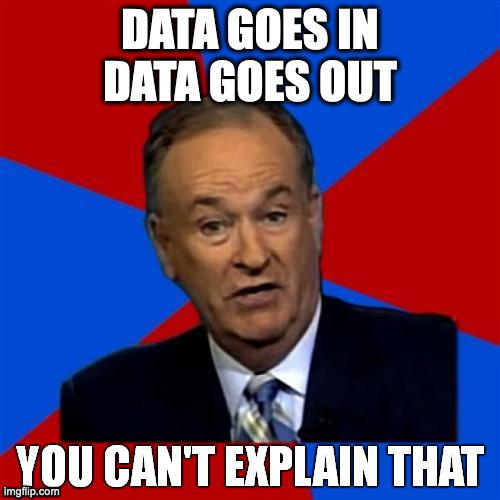
\includegraphics[width=0.3\textwidth]{images/explainthat.jpg}
\end{center}

 \end{frame}



\begin{frame}
\frametitle{Data Models}


 With that in mind, there will be a \alert{data model} -- the abstraction that describes the structure of the database. 
 
 The data model is not only how the database is structured in terms of its schema, but also defines some basic operations to access and modify data.


\end{frame}



\begin{frame}
\frametitle{Data Model Categories}

\begin{itemize}
	\item Relational Model
	\item Entity-Relationship Model
	\item Object-Based Data Model
	\item Semistructured Data Model
\end{itemize}

\end{frame}



\begin{frame}
\frametitle{Entities and Relationships}


We have already discussed the idea of entities as objects. 

A vehicle has a VIN, a year, a model, a colour, et cetera. 

Every vehicle has those attributes, and some of them will be unique (e.g., VIN) to one vehicle and others will be shared.

\end{frame}



\begin{frame}
\frametitle{Entities and Relationships}

In addition to this, we have the concept of a relationship between identities. 

A vehicle is owned by a person. This is a simple association. 

The definition of our associations can also contain some important ``rules'' about our data. 

For example, a vehicle may have only one owner.


\end{frame}



\begin{frame}
\frametitle{Oh no, math!}

To speak more formally about entity relationships we will use some mathematical notation (mostly set notation). 

The relational model traces its way back to a paper published in 1970 that described the database in mathematical relationships and first-order logic. 

\begin{center}
	
\includegraphics[width=0.4\textwidth]{images/math-lady.jpg}
\end{center}

\end{frame}



\begin{frame}
\frametitle{Oh no, math!}

The math may seem intimidating when we first examine it, but ultimately provides an unambiguous and concise way of describing how it all works.

We need to spend some more time to define some terminology, specifically: domain, tuple, attribute, and relation.  

\end{frame}



\begin{frame}
\frametitle{Domain}

A \alert{domain} $D$ is a set of atomic values, where atomic means that the value is not divisible in the relational model. 

Is a phone number like {(212)~867-5309} divisible?

If so, should it be represented in one field? 

\end{frame}



\begin{frame}
\frametitle{The Lack of a Value}

Fields, domains, have a data type associated with them such as integer, string... 

Oftentimes there is a specified length of the field.

To indicate that a value is missing, unknown, or not relevant, there is the possibility for a domain to be \texttt{null}.

Nulls can cause problems... And null does not equal null...

\end{frame}



\begin{frame}
\frametitle{Table = Relation}

In some terminology that might be slightly confusing, a row in a table represents a \alert{relationship} between a set of values 

Things like ``Volkswagen'' and ``Golf'' and ``2015'' all go together. 

This is what we call a \alert{tuple}, which corresponds mathematically with an \textit{n-tuple}.

The table itself we call a \alert{relation}. 

An \alert{attribute} is then a column in that table. 

\end{frame}



\begin{frame}
\frametitle{I warned you there would be math}

A relation schema $R$ is denoted as $R(A_{1}, A_{2}, ..., A_{n})$. 

It is named $R$ and has a list of attributes $A_{1}$ through $A_{n}$. 

Each attribute is the name of a domain $D$. 

The degree of the relation is the number of attributes. 

\end{frame}



\begin{frame}
\frametitle{Table Contents}

The table content, or the relation itself, is denoted $r(R)$ and it is the set of n-tuples where $r = \{t_{1}, t_{2}, ..., t_{m}\}$. 

Each n-tuple is an ordered list of values where each value $v_{i}$ is an element of the domain of attribute $A_{i}$ or the null value. 

We might reference these as $t[A_{i}]$, $t.A_{i}$, or $t[i]$. 

\end{frame}



\begin{frame}
\frametitle{Schema with Data}

\begin{center}
		\textbf{OWNER\_ADDRESS}\\
	\begin{tabular}{|l|l|}\hline
		\textbf{id} & \texttt{integer not null,  primary key}\\ \hline
		\textbf{name} & \texttt{string(64) not null}\\ \hline
		\textbf{street} & \texttt{string(64) not null}\\ \hline
		\textbf{city} & \texttt{string(32) not null}\\ \hline
		\textbf{province} & \texttt{string(2) not null}\\ \hline
		\textbf{postal\_code} & \texttt{string(7) not null}\\ \hline

	\end{tabular}
\end{center}

Then the relation might look something like this:
{\scriptsize
\begin{center}
		\textbf{OWNER\_ADDRESS}\\
	\begin{tabular}{|l|l|l|l|l|l|}\hline
		\textbf{id} & \textbf{name} &\textbf{street} & \textbf{city} & \textbf{province} & \textbf{postal\_code} \\ \hline
		24601 & Jean Valjean & 19 Rue des Prisonniers & Ottawa & ON & B1B 1B1\\ \hline
		25981 & Thomas Anderson & 1234 Main St & Waterloo & ON & A0A 0A0\\ \hline
		12949 & Alice Jones & 4 Generic Place & Kenora & ON & C2C 2C2\\ \hline
	\end{tabular}
\end{center}
}
\end{frame}



\begin{frame}
\frametitle{Defining the Relationship}

A relationship is an association among several entities. 

License and address have a relationship and that relationship we can call ``ownership''.

A relationship set is a mathematical relationship set is a mathematical relation among $n \geq 2$ entities:

\begin{center}
 $\{(e_{1}, e_{2}, ..., e_{n}) | e_{1} \in E_{1}, e_{2} \in E_{2}, ..., e_{n} \in E_{n}\}$
\end{center}

where $(e_{1}, e_{2}, ..., e_{n})$ is a relationship.


\end{frame}



\begin{frame}
\frametitle{Relationships can be messy...}

We might have a rather unwieldy relationship: between vehicle and license there are a lot of columns. 

A license plate is uniquely identified by its numbers and/or letters and a vehicle is uniquely identified by its VIN. 

To prevent redundant (duplicate) data, we prefer that we use just their unique identifiers. 

Example:  (ZZZZ999, 5N1BA0ND5BNF18322)

\end{frame}



\begin{frame}
\frametitle{Relationships as Tables}

The relationship representing ownership will itself be a relation (a table). 

It has two columns: one for the license plate number and one for the VIN. 

\end{frame}



\begin{frame}
\frametitle{Relationships as Tables}

A relationship may possess attributes of its own, that is, ones that do not directly reference the attributes of other relations (tables). 

The relationship may have a third attribute that contains a date and time when the relationship was last modified.

\end{frame}



\begin{frame}
\frametitle{Sometimes Two, There Are}

The most common of relationship is binary: it involves two entity sets 

A particular table may be involved in arbitrarily many relationships. 

\end{frame}



\begin{frame}
\frametitle{Sometimes Two, There Are}

We are not restricted to binary relationships; a relationship between multiple entities can be created. 

If we were to track insurance policies in our database, perhaps?

Sometimes a mapping will not (yet) exist.

\end{frame}



\begin{frame}
\frametitle{Constraints}

In the relational model we call restrictions or rules constraints.

Categories of constraints:

\begin{enumerate}
\item Constraints inherent in the data model.
\item Explicitly added constraints.
\item Constraints that cannot be captured in the data model. 
\end{enumerate}

\end{frame}



\begin{frame}
\frametitle{Rule Problems}

Some constraints, unfortunately, cannot be described in the data model. 

There is no good way to specify the format must follow the Canadian postal code format (e.g., A1B2C3). 

\begin{center}
	
\includegraphics[width=0.3\textwidth]{images/therules.jpg}
\end{center}

These constraints, if they are to be enforced, must be enforced outside of the database. Such things are sometimes called business rules.


\end{frame}




\begin{frame}
\frametitle{Cardinality Constraints}

\begin{center}
	
\includegraphics[width=0.3\textwidth]{images/cardinal.jpg}
\end{center}

Cardinality constraints express relationships in a structured way. Our choices: 

\begin{itemize}
\item One to one (1:1).
\item One to many (1:N).
\item Many to one (N:1).
\item Many to many (N:M).
\end{itemize}

\end{frame}



\begin{frame}
\frametitle{Keys are Key}

We need a way to identify tuples uniquely in terms of their attributes. 

That is to say, no two tuples in the table are permitted to be exactly the same in every column. 

A \alert{super key} is a set of one or more attributes that uniquely identify one tuple in the relation (table).

\end{frame}

\begin{frame}
\frametitle{Keys are Key}

By default, of course, the full set of attributes will be one such super key. 

Some attributes on their own will be a super key, such as VIN; VINs are unique.

Others are not: names are not unique. 

But a super key may be something like (VIN, make, model). 

\end{frame}



\begin{frame}
\frametitle{Small Keys}

If a super key is as small as it can be but no smaller, then it is a minimal super key and we call it a \alert{candidate key}. 

A candidate key, more formally, has no proper subset that is a super key. 

(VIN, make, model) is a super key but not a candidate key;\\
\quad VIN on its own is a candidate key.

\end{frame}



\begin{frame}
\frametitle{Multiple Candidates}

There are then, potentially, several candidate keys. 

A student at the University of Waterloo can be identified uniquely by both a student number (e.g., 20000000) and a userid (j9999doe). 

Both of those are candidate keys for identifying an individual student. 

The database designer will choose a \alert{primary key} from the candidates to be the main way of uniquely identifying a tuple. 


\end{frame}



\begin{frame}
\frametitle{Electing a Candidate}

Soon enough we will spend some time to discuss good database design. 

Typically, the primary key will be one field, to reduce duplication and confusion. 

We've seen a little bit of that already in that we assigned addresses an ``ID'' field. 

A primary key should be something that is always present and always unique.

\end{frame}

\begin{frame}
\frametitle{Join Relation}

\begin{center}
	
\includegraphics[width=0.7\textwidth]{images/join.jpg}
\end{center}


\end{frame}


\begin{frame}
\frametitle{Join Relation}

When we have a join relation the primary key may be formed by the two entities being referenced. 

If the relation has a tuple (ZZZZ999, 5N1BA0ND5BNF18322) then that itself can be the primary key. 

Or if we have a list of elements belonging to some parent, they might be identified uniquely by the parent's ID and an integer sequence number.

\end{frame}




\begin{frame}
\frametitle{Primary Key Implications}

Keep in mind that a primary key means no two tuples can have the same values for that attribute (or those attributes) at the same point in time. 

Suppose we have a relation where the primary key is the parent's ID and the sequence number. 

Tuples like (92858, 0, Smith), (92858, 1, Kim), (92858, 2, Singh), where the first two elements form the primary key. 

Suppose we then delete the first element of the sequence:\\
\quad The tuples are now (92858, 0, Kim), (92858, 1, Singh). 

This is okay!

\end{frame}



\begin{frame}
\frametitle{Foreign Keys}

If a relation references the primary key of another, we can make it a requirement that its content matches an entry in the domain of another table. 

When a vehicle row is created, the license plate number must be one of the entries in the license plate table (or null, if that is permitted).

Thus, if we tried to put in an entry that referenced license plate ``DDDD 001'' when no such plate exists in the system, this would be an error. 

This explicit constraint is called a \alert{foreign key}. 


\end{frame}



\begin{frame}
\frametitle{Foreign Key}

More formally, a foreign key is defined as:
\begin{enumerate}
\item The attributes of the foreign key of relation $R_{1}$ relating $R_{1}$ to relation $R_{2}$ have the same domain(s) as the primary key of $R_{2}$.
\item A value of a FK in a tuple $t_{1}$ of $R_{1}$ either occurs as a value of the primary key for some tuple $t_{2}$ in $R_{2}$ in the current state, or is null. 
\end{enumerate}

A foreign key is also called a referential integrity constraint.

\end{frame}



\begin{frame}
\frametitle{Reject}

Under best circumstances, the database server will reject any attempt to modify data such that violates referential integrity (or otherwise breaks a rule). 

If that is so, we may have some certainty that our data is in a valid state. 

If there are rules not entered into the system explicitly at the beginning it may be very painful to introduce them later if the system is in an invalid state. 


\end{frame}



\begin{frame}
\frametitle{``University'' Schema}

\begin{center}
	\includegraphics[width=\textwidth]{images/schemadiagram.png}
\end{center}


\end{frame}




\end{document}

